\section{Smart Darts}\label{sec:SmartDarts}

\subsection{Design}
The Smart dart combines a geophone \todo{(model number)} with the fins and body of a lawn Jart (TM), using a 3D-printed chamber that encloses a photo cellular-enabled microcontorller (link).

This design was selected because of (blah blah)

The following sections compare the performance of the Smart Darts in different soils, 



\subsection{Experiments}
\subsubsection{ Drop tests in different soils} 
This experiment varied the drop height and measured the penetration depth in four types of soil.
Proper planting of a geophone requres godd contact by ensuring the geophone is pushed deep into the soil, and the sensors should be close to vertical because accelerometers
deviation from 
 to determine the minimum height for
Each trial measured the penetration depth and the angular error from vertical.
This experiment compared drop tests as function of soil type.  
Results are summarized in Fig.~\ref{fig:DepthPlotIndoors}, which shows penetration depth, and Fig.~\ref{fig:AnglePlotIndoors}, which shows angle of defication.

Soil types are calibrated using a handheld penetrometer \todo{(model number)}

\begin{figure} \centering
{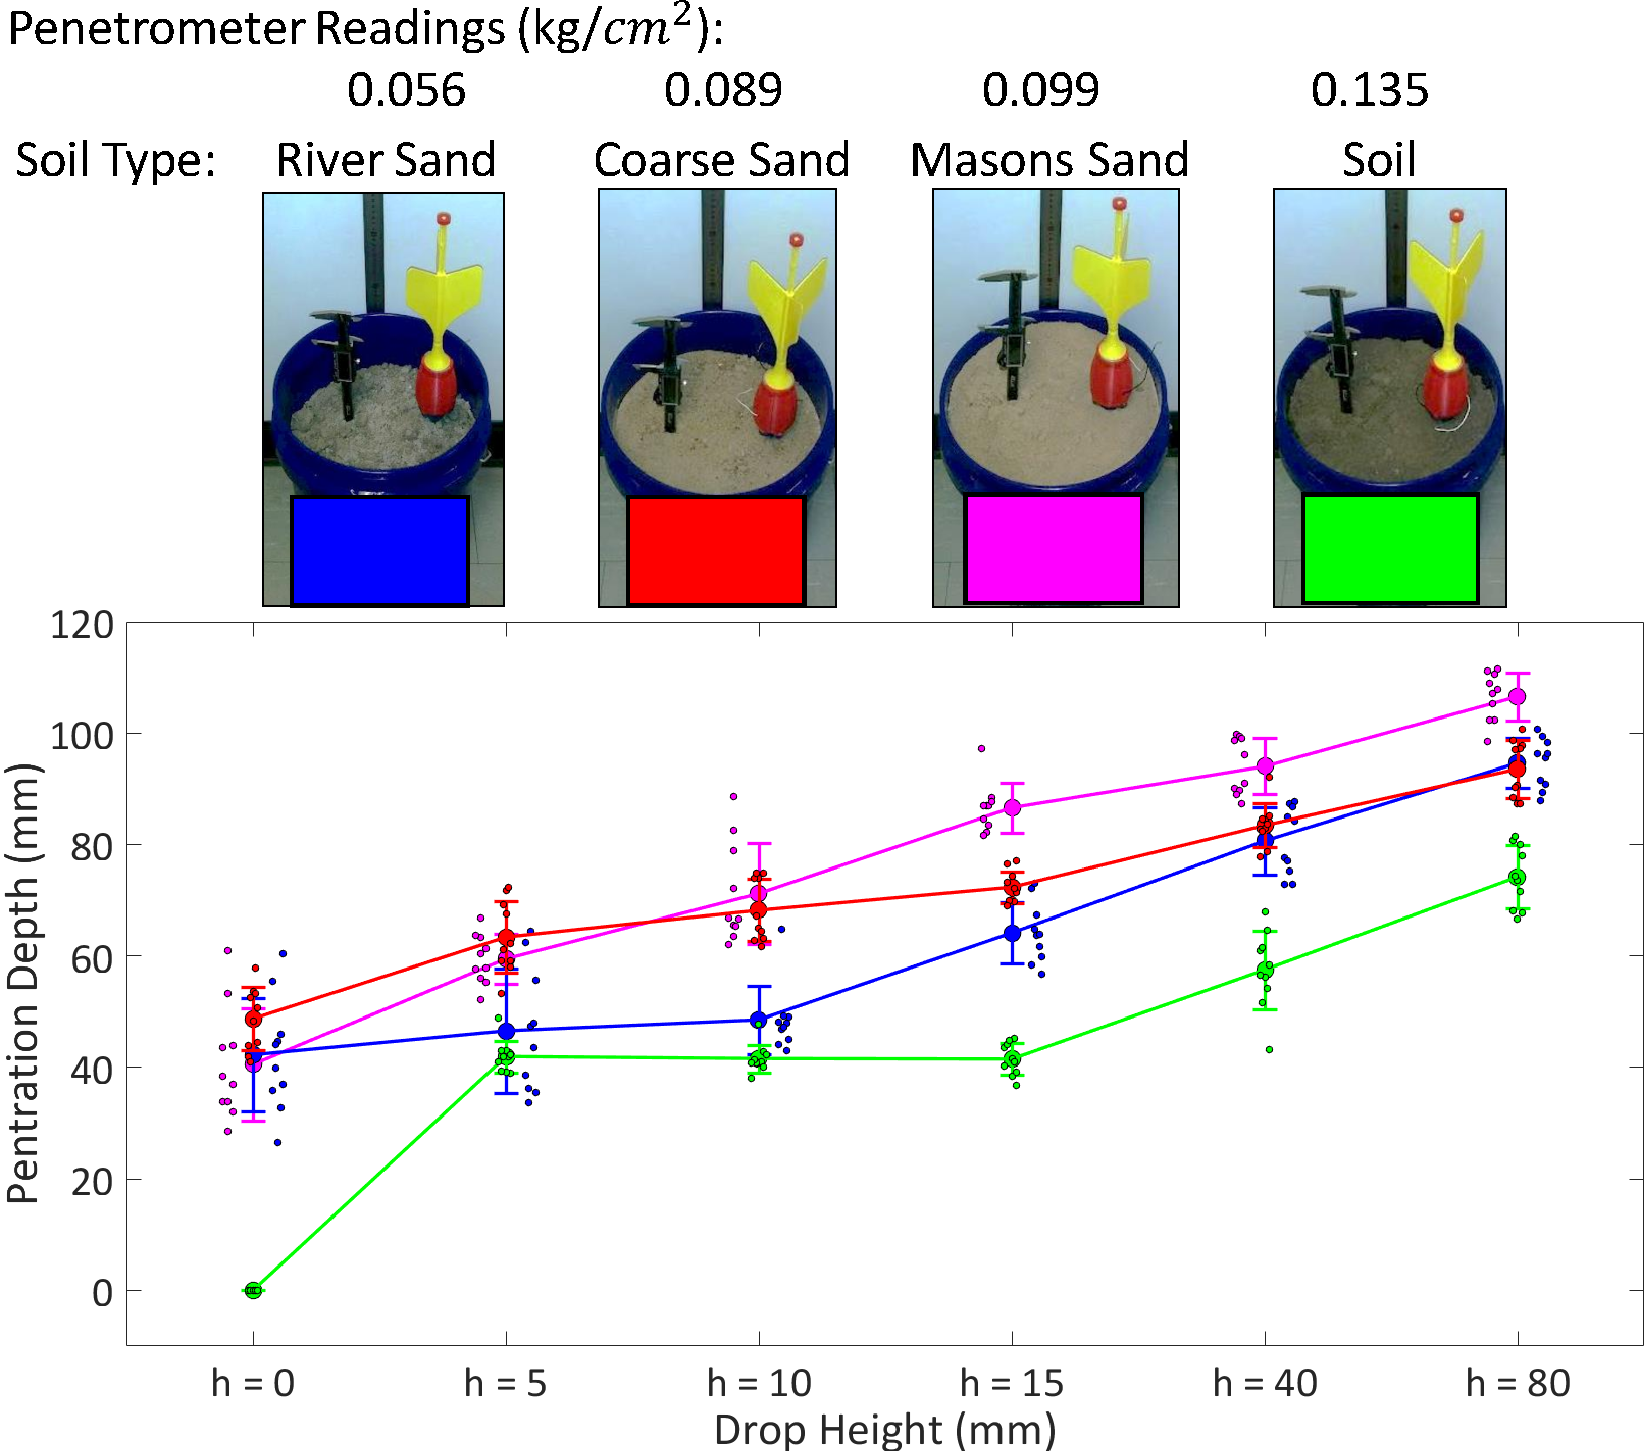
\includegraphics[width=\columnwidth]{indoor_depth_plot.pdf}}
\caption{Drop height vs. penetration depth in four soil types.} 
\label{fig:DepthPlotIndoors}
\end{figure}

\begin{figure} \centering
{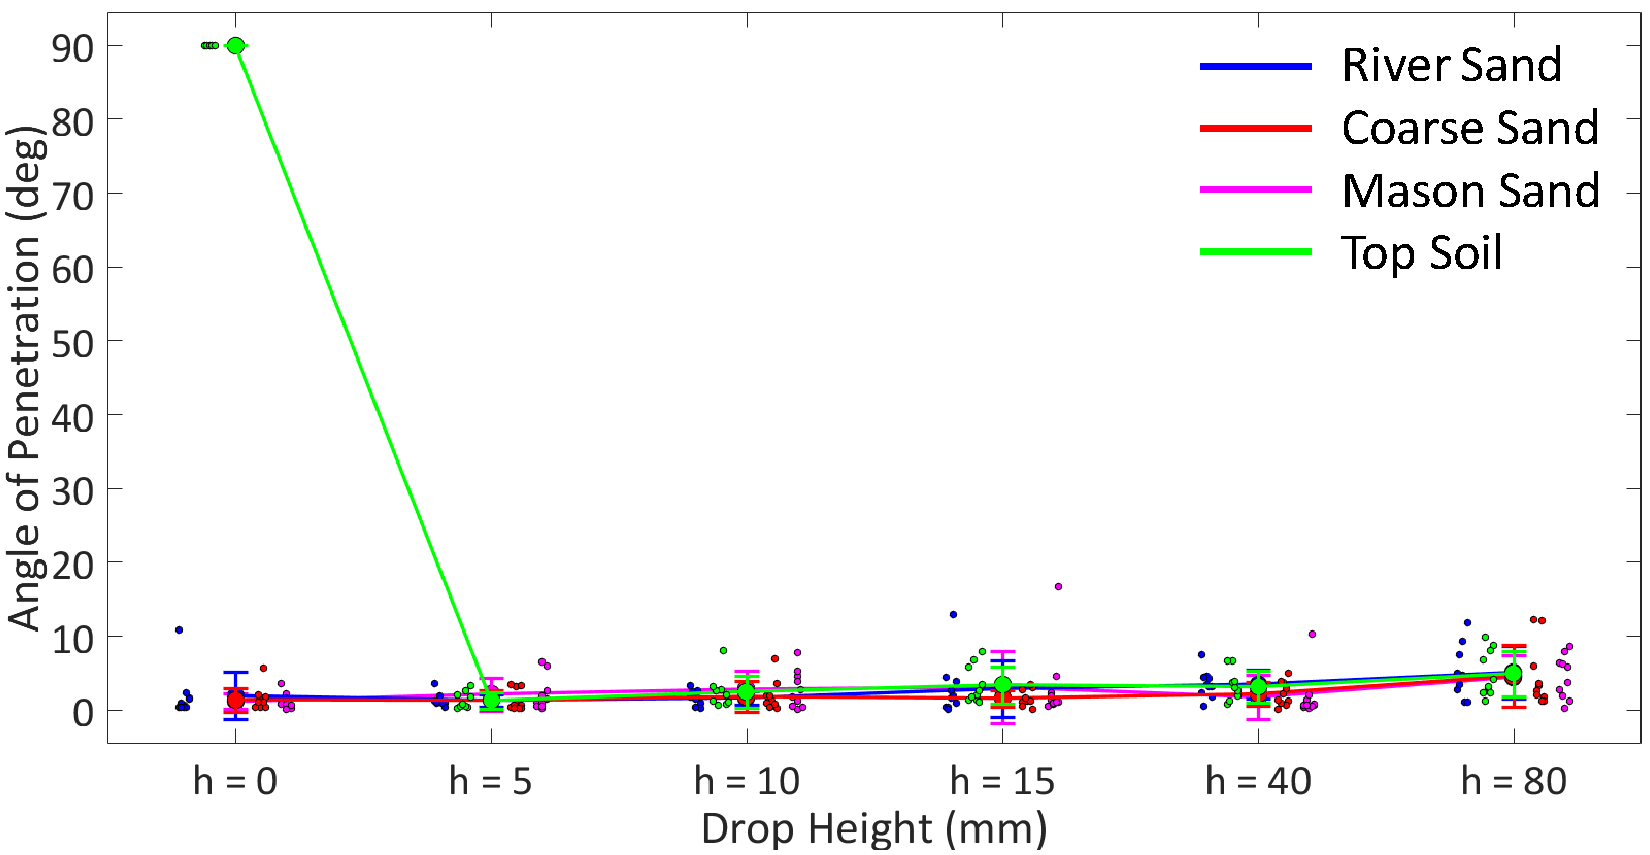
\includegraphics[width=\columnwidth]{indoor_angle_plot.pdf}}
\caption{Drop height vs. angle of deviation in four soil types.} 
\label{fig:AnglePlotIndoors}
\vspace{-1em}
\end{figure}

\subsubsection{Straight vs Bent Fins}

Drop tests as function of height. Compares depth and angle for twisted vs. straight tail.
Results are summarized in Fig.~\ref{fig:StraightBentPic}.

\begin{figure} \centering
  {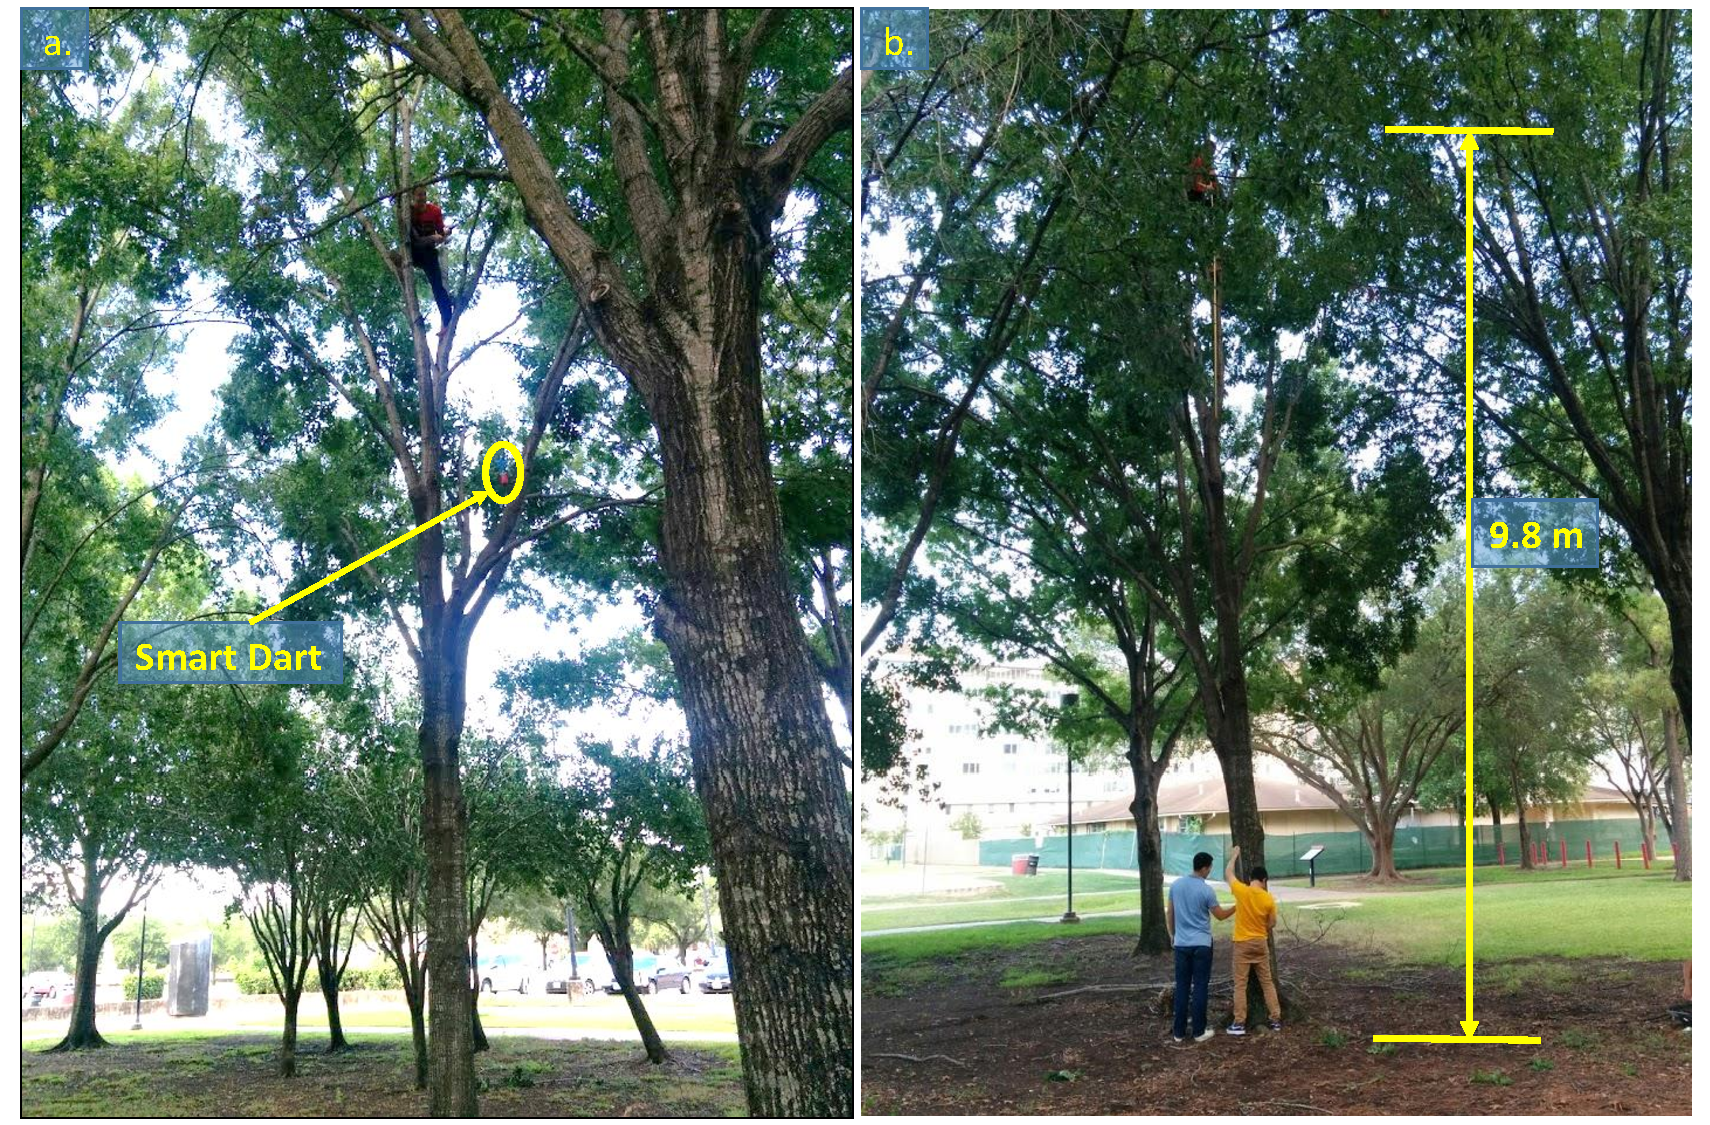
\includegraphics[width=\columnwidth]{StraightBentPic.pdf}}
 \caption{Outdoor Drop test comparing Straight vs Bent fins performance.
 a.)  smart dart dropping 
 b.)  measuring drop height} 
 \label{fig:StraightBentPic}
 \vspace{-1em}
\end{figure}
\begin{figure} \centering
  {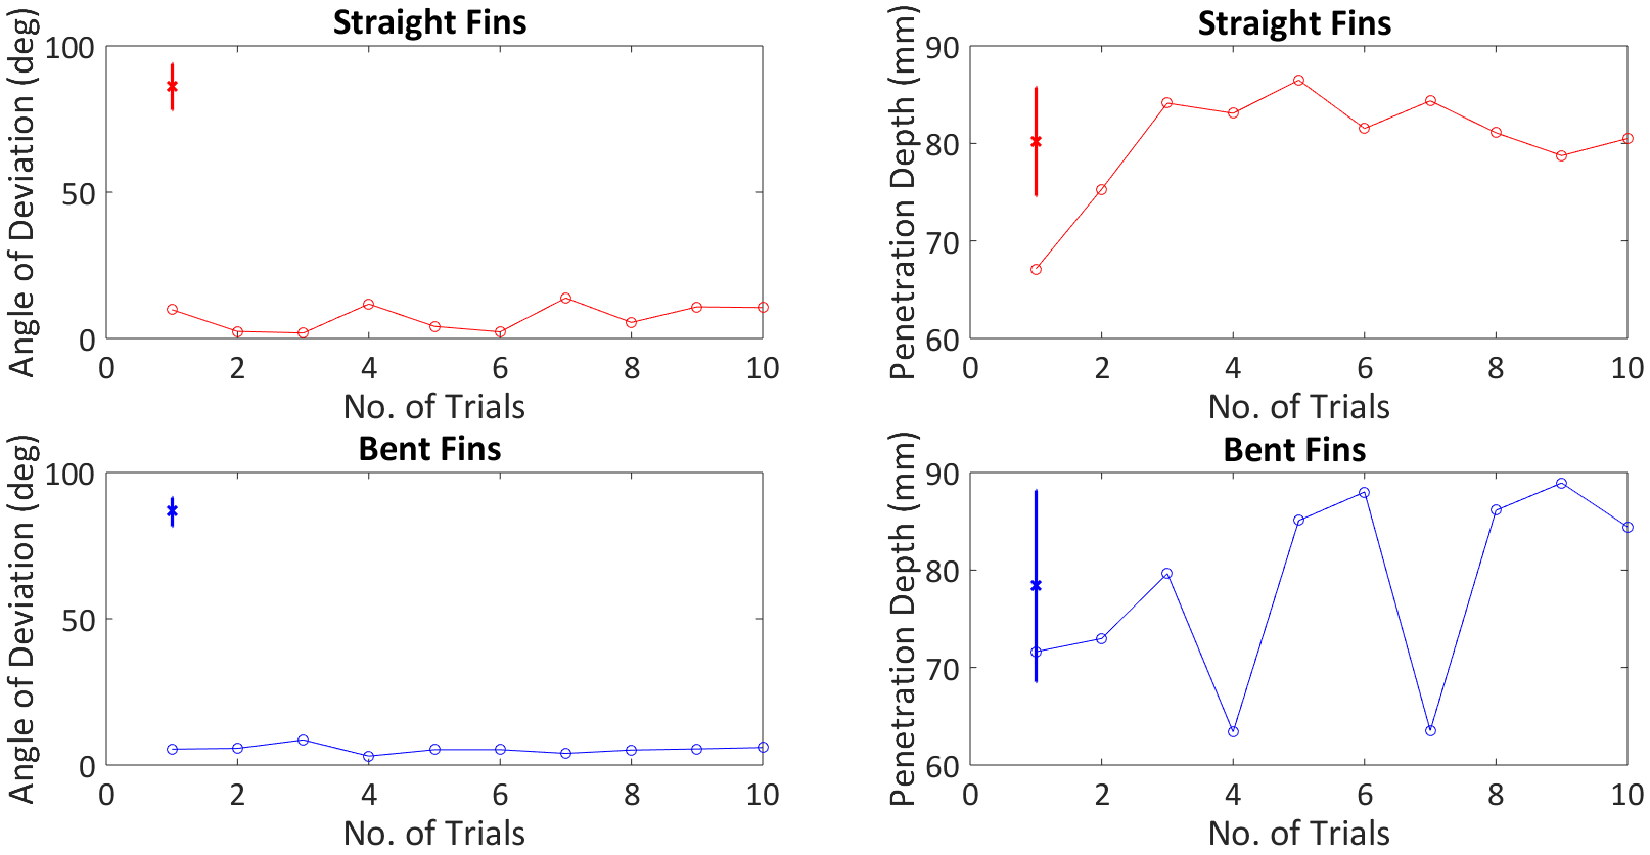
\includegraphics[width=\columnwidth]{StraightBentPlot.pdf}}
 \caption{Straight vs Bent fins comparing penetration depth and angle of deviation. Experiment used a fixed drop height of 9.8 m.} 
 \label{fig:StraightBentPlot}
\end{figure}



\subsubsection{Shot gather comparison}
Exp 3: Dart sensing accuracy vs ground setup

\todobox{Srikanth:  Need figure for accuracy of placement for drone drop}

 